\documentclass[aspectratio=169]{beamer}
\usepackage{color,amsmath}
\usepackage{subfigure}
\usepackage{booktabs}
\usepackage{framed}
\usepackage{comment}
\usepackage{url}

\hypersetup{
    colorlinks=true,
    linkcolor=blue,
    filecolor=magenta,      
    urlcolor=cyan,
}


%%%%%%%%%%%%%%%%%%%%%%%%%%
\title[]{Introduction to group activity}
\author[]{Matthew J. Salganik\\Department of Sociology\\Princeton University}
\date[]{Summer Institutes in Computational Social Science\\June 20, 2019
\vfill
\begin{flushleft}
{\scriptsize
The Summer Institutes in Computational Social Science is supported by grants from the Russell Sage Foundation and the Alfred P. Sloan Foundation.}
\end{flushleft}
\begin{flushright}

\includegraphics[width=0.1\textwidth]{figures/cc-by.png}
\end{flushright}
}
\begin{document}
%%%%%%%%%%%%%%%%%%%%%%%%%%
\frame{\titlepage}
%%%%%%%%%%%%%%%%%%%%%%%%%%
\begin{frame}

\begin{center}
\only<1>{
\includegraphics[width=0.9\textwidth]{figures/goel_online_2017_title}}
\only<2>{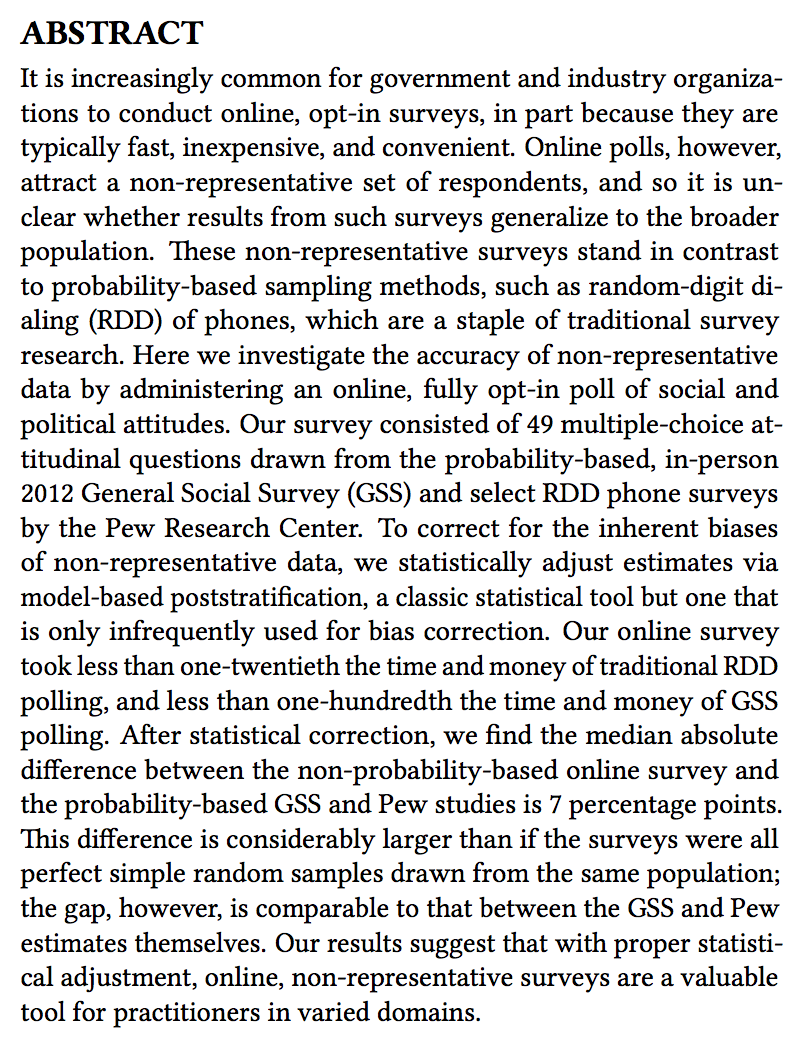
\includegraphics[width=0.4\textwidth]{figures/goel_online_2017_abstract}}
\end{center}

\vfill
\url{https://5harad.com/papers/dirtysurveys.pdf}

\end{frame}
%%%%%%%%%%%%%%%%%%%%%%%%%%%
\begin{frame}

Activity:
\begin{itemize}
\item Design a questionnaire using questions already asked on high quality surveys
\pause
\item Recruit participants from Amazon Mechanical Turk and have them complete your questionnaire  
\pause
\item Compare results from your survey to the results from the high-quality survey
\pause
\item Try different approaches to weighting and see how the change the estimates
\pause
\item De-identify and ``open-source'' data by sending to your local organizer (but remember to think about the end at the beginning)
\end{itemize}

\end{frame}
%%%%%%%%%%%%%%%%%%%%%%%%%%
\begin{frame}

This activity will give you practice:
\begin{itemize}
\item Designing questionnaires
\pause
\item Collecting survey data
\pause
\item Analyzing survey data (data wrangling and post-stratification)
\pause
\item Using the total survey error framework to consider and discussion errors in estimates
\pause
\item Working with Amazon Mechanical Turk
\pause
\item Archiving data for other researchers
\end{itemize}

\vfill
Remember: This is a learning activity so try whatever you want.

\end{frame}
%%%%%%%%%%%%%%%%%%%%%%%%%%%
\begin{frame}

Our recommended work flow:
\begin{itemize}
\item Create a write-up that describes what data you will be collecting, why, and how it will be shared with others (for tips, see \href{https://doi.org/10.1177/2515245917747656}{Meyer})
\end{itemize}

\end{frame}
%%%%%%%%%%%%%%%%%%%%%%%%%%
\begin{frame}

Our recommended work flow:
\begin{itemize}
\item Create a write-up that describes what data you will be collecting, why, and how it will be shared with others (for tips, see \href{https://doi.org/10.1177/2515245917747656}{Meyer})
\item Create survey on Google Forms (we have a \href{https://github.com/compsocialscience/summer-institute/blob/master/2019/materials/day4-surveys/activity/2019-06-13_mturk_google_survey.pdf}{template})
\end{itemize}

\end{frame}
%%%%%%%%%%%%%%%%%%%%%%%%%%
\begin{frame}

\begin{center}
\begin{tabular}{ccc}
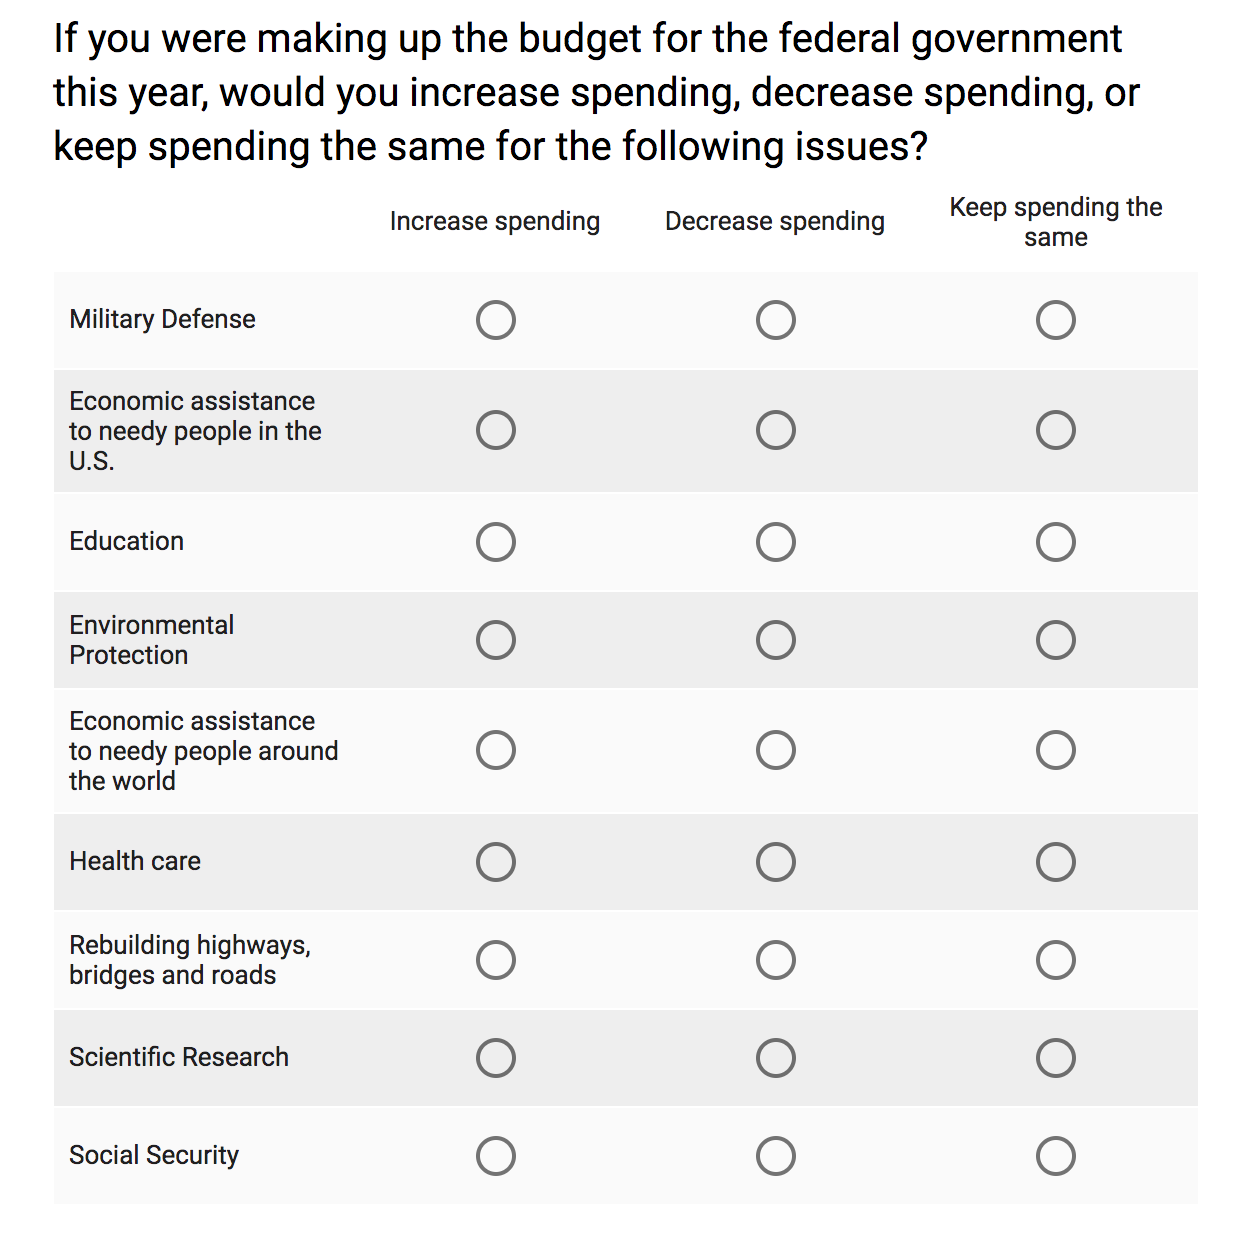
\includegraphics[width=0.30\textwidth]{figures/MTurk_survey_grid} & \phantom{12} \LARGE{or} \phantom{12}  & 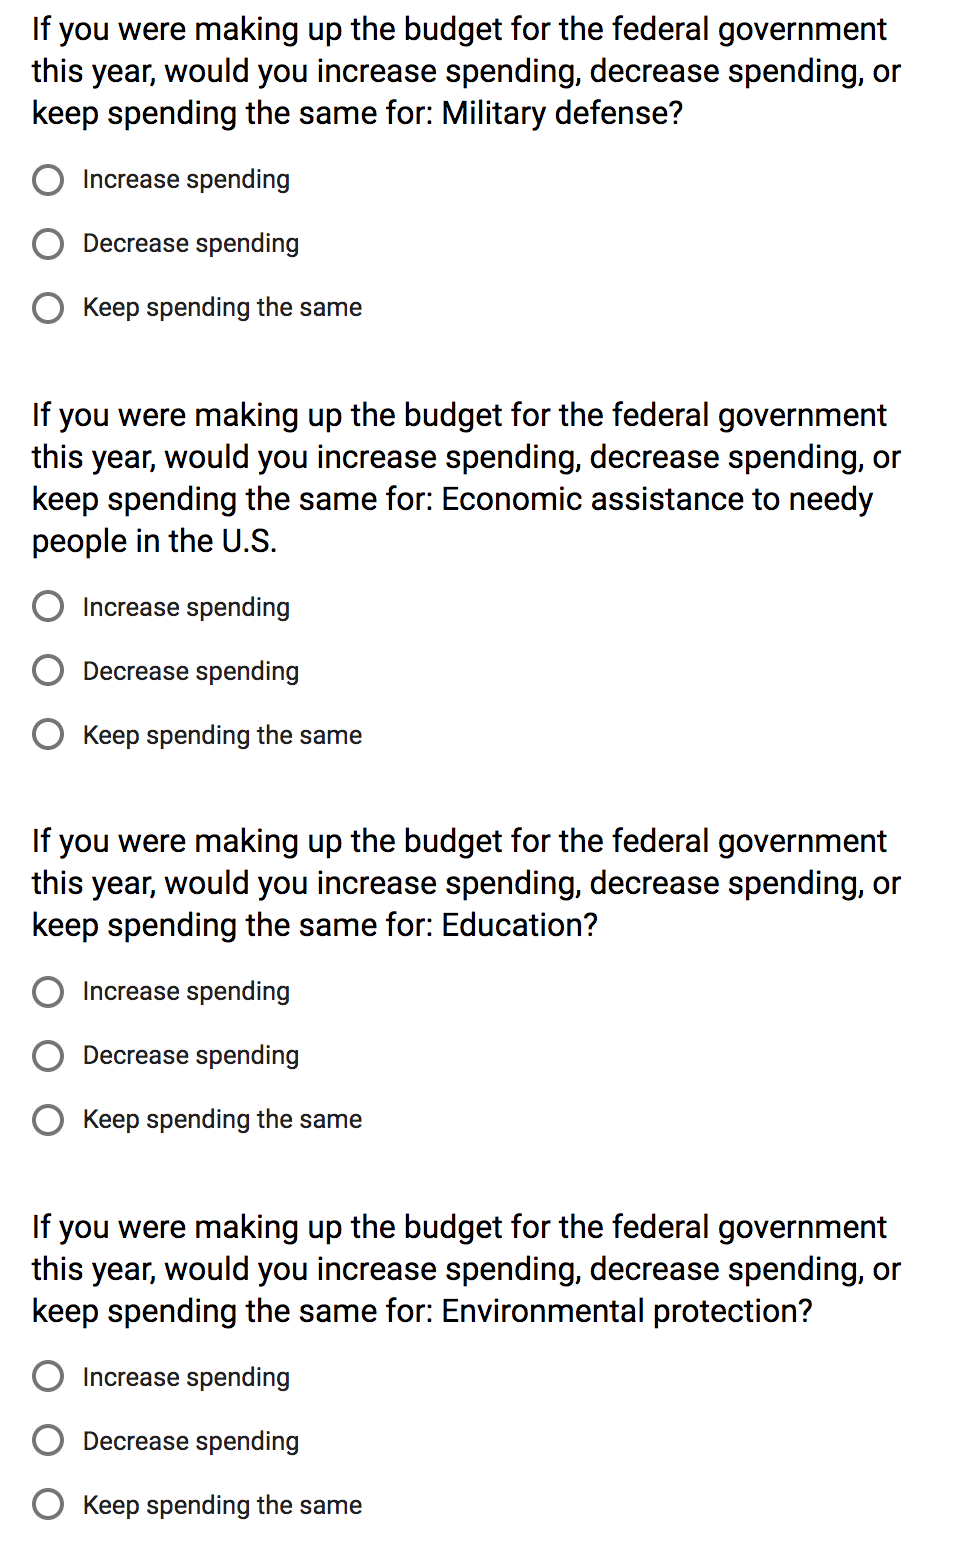
\includegraphics[width=0.30\textwidth]{figures/MTurk_survey_list}
\end{tabular}
\end{center}

\end{frame}
%%%%%%%%%%%%%%%%%%%%%%%%%%
\begin{frame}

Don't forget to collect the information that you will need for post-stratification: \pause
\begin{itemize}
\item gender
\item age
\item state of residence
\item race/ethnicity
\end{itemize}

How should you ask these questions?  \pause You should copy from the American Community Survey.

\end{frame}
%%%%%%%%%%%%%%%%%%%%%%%%%%
\begin{frame}

Our recommended work flow:
\begin{itemize}
\item Create a write-up that describes what data you will be collecting, why, and how it will be shared with others (for tips, see \href{https://doi.org/10.1177/2515245917747656}{Meyer})
\item Create survey on Google Forms (we have a \href{https://github.com/compsocialscience/summer-institute/blob/master/2019/materials/day4-surveys/activity/2019-06-13_mturk_google_survey.pdf}{template})
\pause
\item Deploy to MTurk
\end{itemize}

\end{frame}
%%%%%%%%%%%%%%%%%%%%%%%%%%
\begin{frame}

\begin{center}
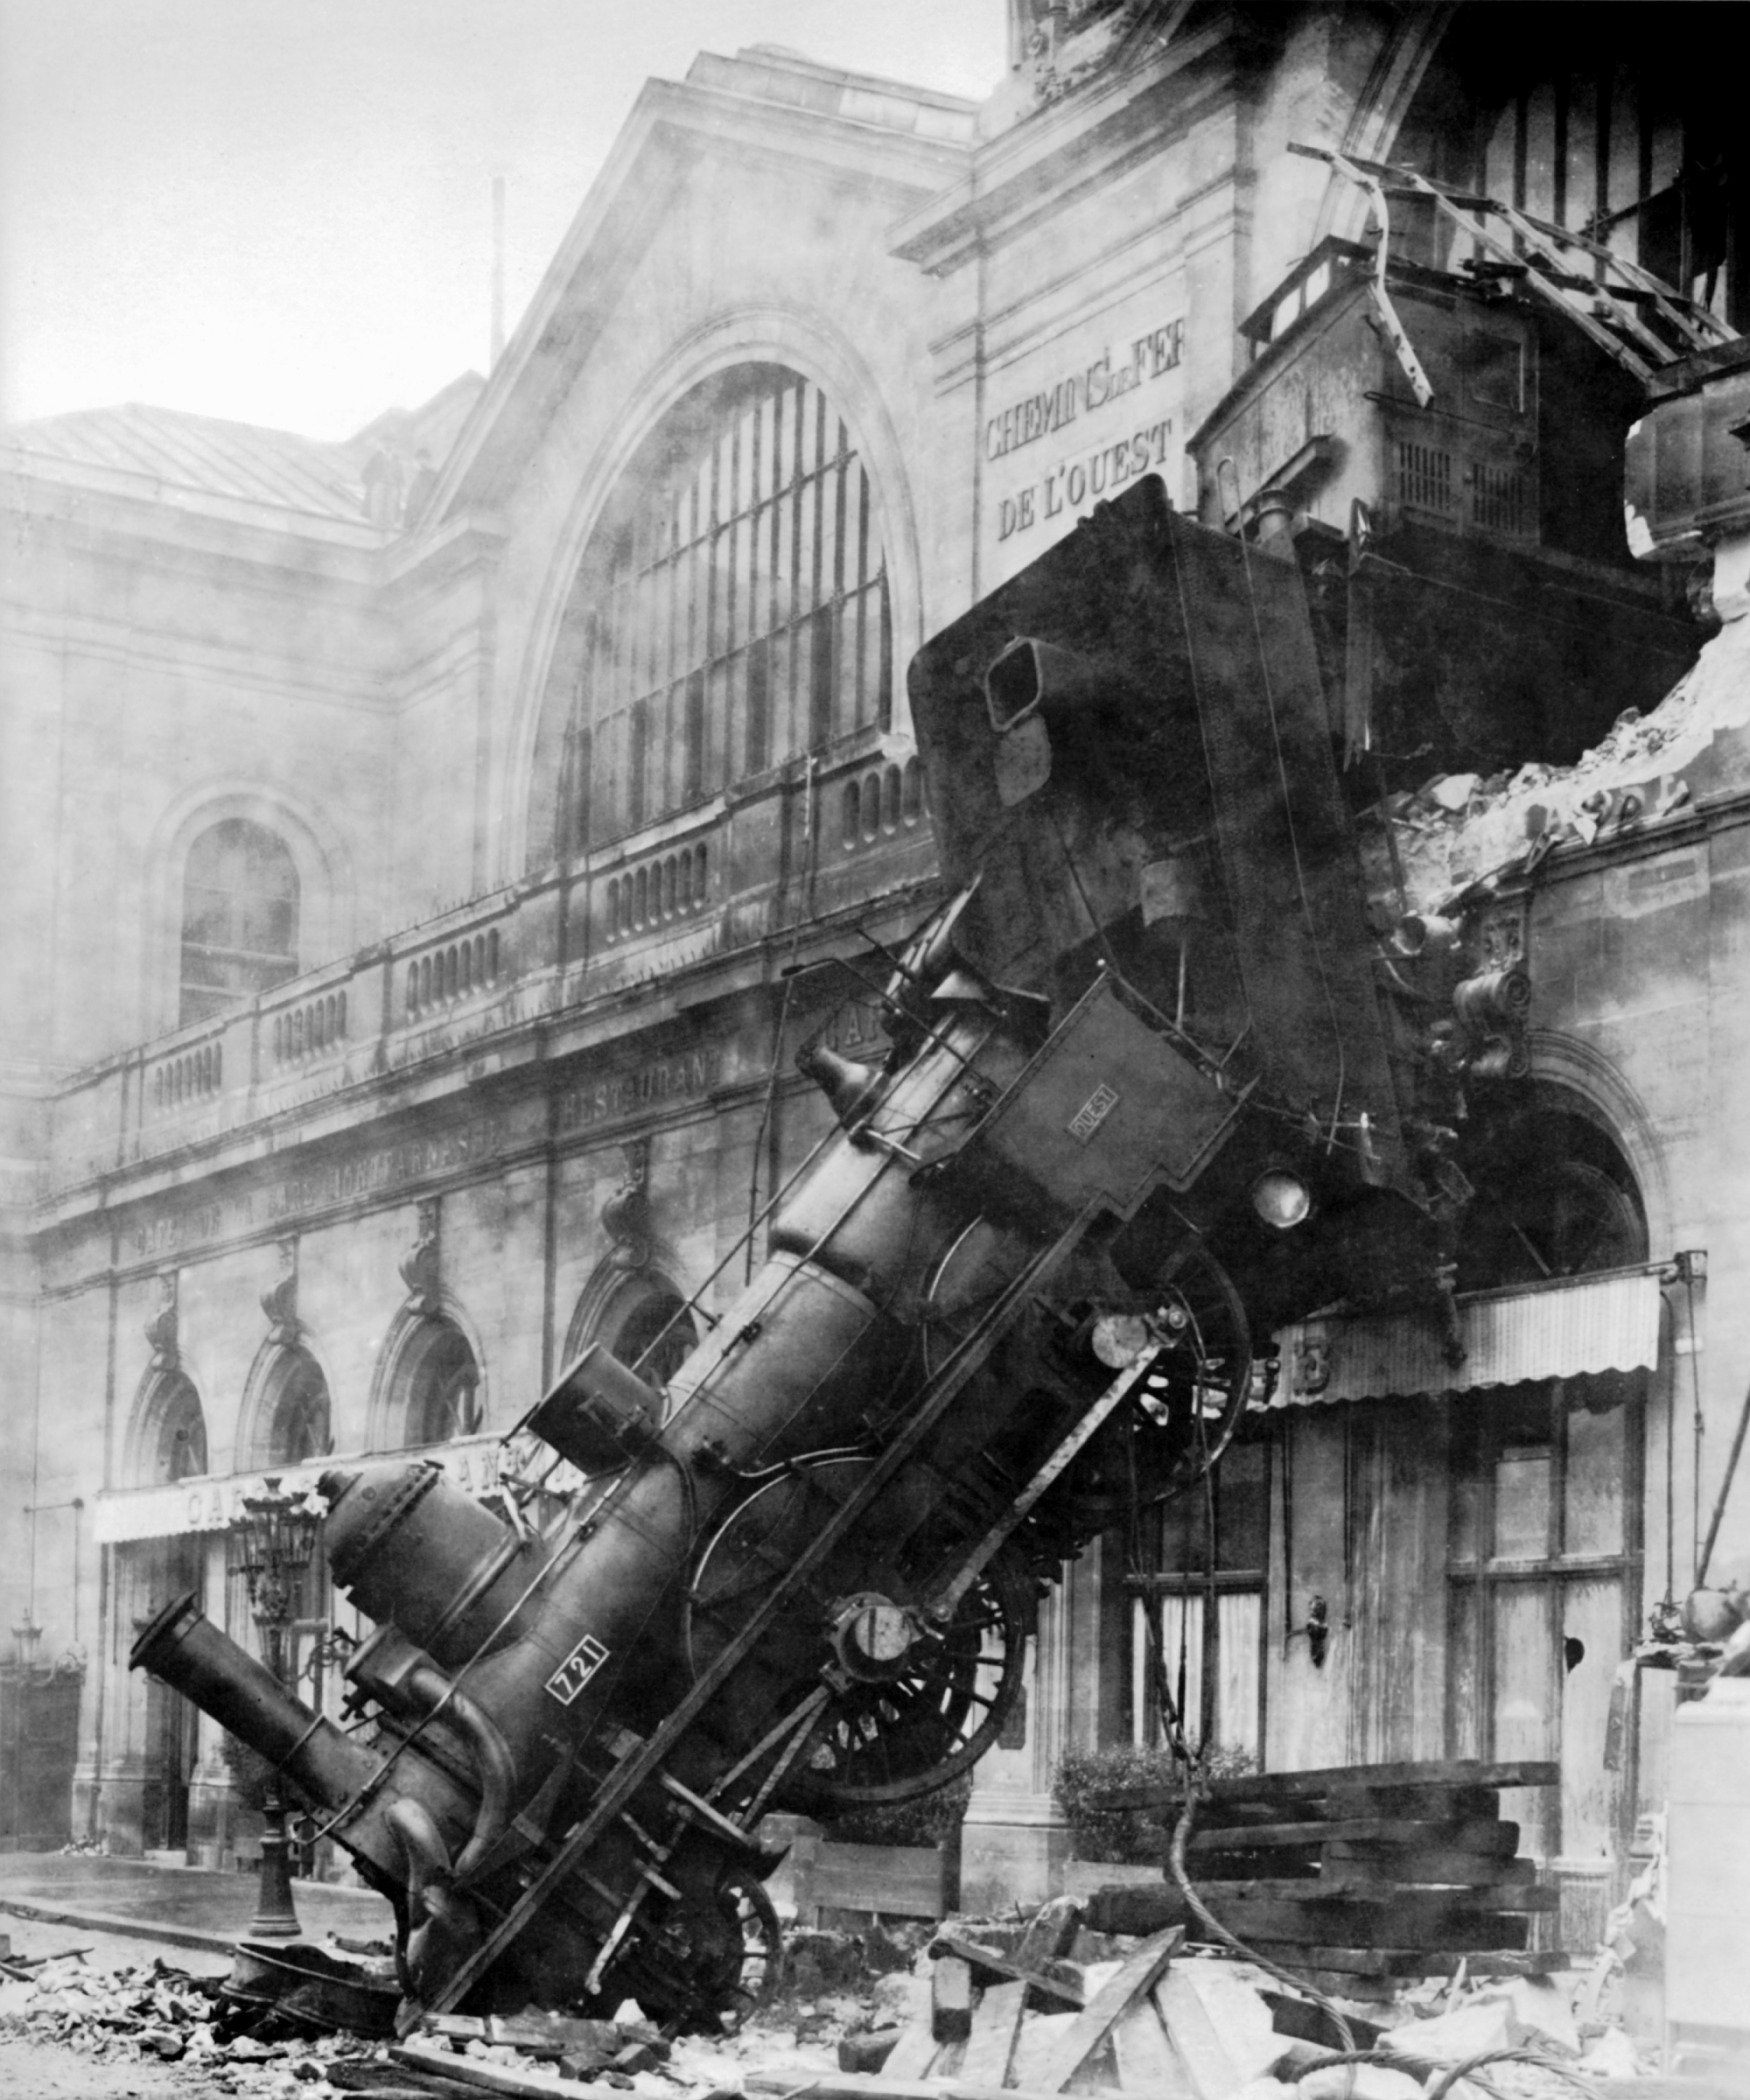
\includegraphics[height=0.6\textheight]{figures/Train_wreck_at_Montparnasse_1895.jpg}
\end{center}

Last year, every group made at least one error deploying their relatively simple survey.

\vfill

{\tiny \url{https://en.wikipedia.org/wiki/Failure\#/media/File:Train_wreck_at_Montparnasse_1895.jpg}}
\end{frame}
%%%%%%%%%%%%%%%%%%%%%%%%%%
\begin{frame}

Our recommended work flow:
\begin{itemize}
\item Create a write-up that describes what data you will be collecting, why, and how it will be shared with others (for tips, see \href{https://doi.org/10.1177/2515245917747656}{Meyer})
\item Create survey on Google Forms (we have a \href{https://github.com/compsocialscience/summer-institute/blob/master/2019/materials/day4-surveys/activity/2019-06-13_mturk_google_survey.pdf}{template})
\item Deploy to MTurk
\pause
\item Take a break
\end{itemize}

\end{frame}
%%%%%%%%%%%%%%%%%%%%%%%%%%
\begin{frame}

\begin{center}
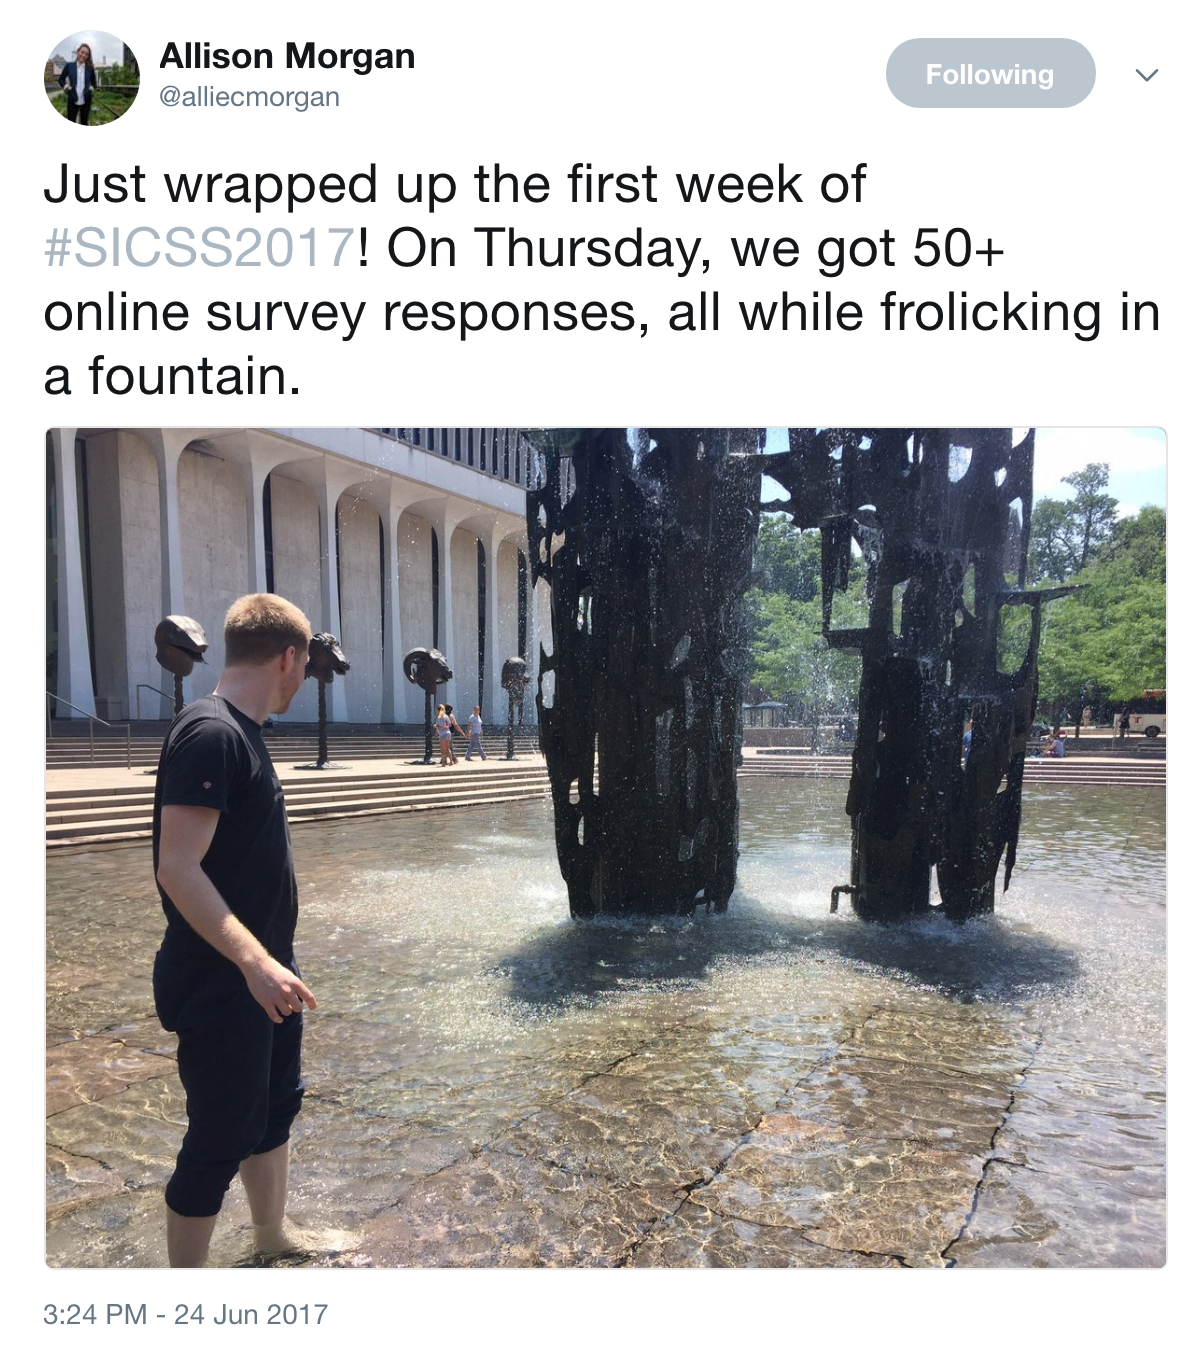
\includegraphics[width=0.4\textwidth]{figures/morgan_tweet}
\end{center}

\end{frame}
%%%%%%%%%%%%%%%%%%%%%%%%%%
\begin{frame}

Our recommended work flow:
\begin{itemize}
\item Create a write-up that describes what data you will be collecting, why, and how it will be shared with others (for tips, see \href{https://doi.org/10.1177/2515245917747656}{Meyer})
\item Create survey on Google Forms
\item Deploy to MTurk
\item Take a break
\pause
\item Validate and pay workers
\pause
\item Analyze the much larger sample that we have collected for you
\end{itemize}

\end{frame}
%%%%%%%%%%%%%%%%%%%%%%%%%%
\begin{frame}

A quick and dirty tour of the post-stratification methods we will use

\end{frame}
%%%%%%%%%%%%%%%%%%%%%%%%
\begin{frame}

Use this estimator in three steps:
\begin{enumerate}
\item Chop up the sample into groups \pause
\item Estimate the mean in each group \pause
\item Combine the estimates for each group into an overall estimate
\end{enumerate}
\pause

\vfill

\begin{equation*}
\hat{\bar{y}}_{post} = \sum_{h=1}^H \frac{N_h}{N} \hat{\bar{y}}_h
\end{equation*}
where 
\begin{itemize}
\item $N$: size of the population
\item $N_h$: size of group $h$
\item $\hat{\bar{y}}_h$: estimated average outcome for group $h$
\end{itemize}

\end{frame}
%%%%%%%%%%%%%%%%%%%%%%%%
\begin{frame}
\frametitle{Cell-based Poststratification}

Assumptions:
\begin{itemize}
\item The realized sample $s$ is partitioned into $H$ groups, $s_1, s_2, \ldots s_H$
\item Given $s$, all elements in $s_k$ are assumed to have the same response probability; different groups can have different response probabilities
\item Equivalent to data is missing completely at random (MCAR) within each group
\item ``Response Homogeneity Group Model'' (RHG Model), see Sarndal et al.\ (1992) Sec 15.6.2 (``A Useful Response Model'')
\end{itemize}

\vfill
If RHG model holds (and some other minor technical conditions), then the poststratification estimator is unbiased.  See Sarndal et al.\ (1992) Result 15.6.1 

\end{frame}
%%%%%%%%%%%%%%%%%%%%%%%%
\begin{frame}
\frametitle{Bias of cell-based poststratification estimator from non-response}

If RHG does not hold and if the original sample is simple random sampling without replacement, then (Bethlehem, Cobben, and Schouten 2011, sec. 8.2.1):

$$bias(\hat{\bar{y}}_{post}) = \frac{1}{N} \sum_{h=1}^H \frac{cor(\phi_i, y_i)^{(h)} S(\phi_i)^{(h)} S(y_i)^{(h)}}{\bar{\phi}^{(h)}}$$

So, how should we create the $H$ groups? \pause
\begin{itemize}
\item form homogeneous groups where there is little variation in response propensity $(S(\phi_i)^{(h)} \approx 0)$ and the outcome $(S(y_i)^{(h)} \approx 0)$ \pause
\item form groups where the people that you see are like the people that you don't see $(cor(\phi_i, y_i)^{(h)} \approx 0)$
\end{itemize}

\vfill
In practice this can be difficult because you want to form many groups, but then you have noisy estimates for each group.

\end{frame}
%%%%%%%%%%%%%%%%%%%%%%%%
\begin{frame}

Note:
\begin{itemize}
\item Horvitz-Thompson estimation is individual-based weight
\item Poststratification can better be understood as a group-based weight
\end{itemize}

\end{frame}
%%%%%%%%%%%%%%%%%%%%%%%%
\begin{frame}

Three increasingly sophisticated ways to make group estimate $\hat{\bar{y}}_h$.  You won't have time to do all of these:
\begin{itemize}
\item cell-based poststratification
\item model-based poststratification
\item multilevel regression postratification (Mr. P)
\end{itemize}

\end{frame}
%%%%%%%%%%%%%%%%%%%%%%%%
\begin{frame}{Data}

\begin{itemize}
\item Our survey data comes from a survey of 495 people on MTurk collected in less than a week ago
\item We will compare to high-quality telephone surveys from the Pew Research Center (links to \href{https://github.com/compsocialscience/summer-institute/blob/master/2019/materials/day4-surveys/activity/2019_pew_benchmark_data.csv}{questionnaires})
\item To poststratify our survey data, we will use data from the American Community Survey about the population of the US
\item We use multiple questions because estimates are also a property of a question not just a sample.
\end{itemize}

\end{frame}
%%%%%%%%%%%%%%%%%%%%%%%%
\begin{frame}{Data}

Some questions have multiple choice answers, but we convert to a series of binary variables for analysis.  As asked:
\begin{center}
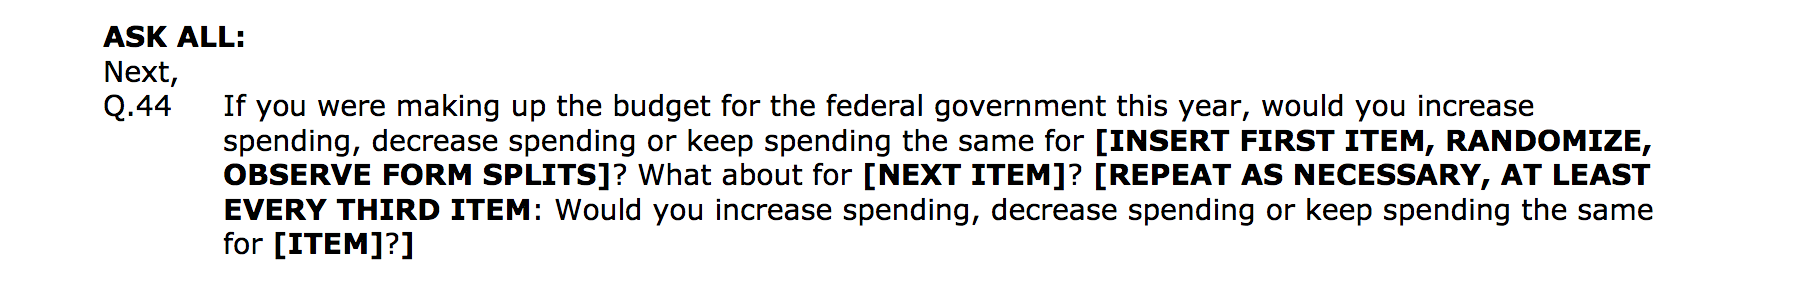
\includegraphics[width=0.8\textwidth]{figures/question_text_pew}
\end{center}

As analyzed:
\begin{itemize}
\item If you were making up the budget for the federal government this year would you increase funding for scientific research?
\item If you were making up the budget for the federal government this year would you decrease funding for scientific research?
\item If you were making up the budget for the federal government this year would you keep funding the same funding for scientific research?
\end{itemize}

\vfill
This means that each of our estimates are not independent.  For real research, you'd want to handle this a different way.

\end{frame}
%%%%%%%%%%%%%%%%%%%
\begin{frame}{Simple cell-based poststratification}

Let's do lots of groups.
\begin{itemize}
\item gender (2 groups)
\item age (4 groups)
\item race (5 groups)
\item region (4 groups)
\item Makes 160 $(2 \times 4 \times 5 \times 4)$ groups
\end{itemize}

\end{frame}
%%%%%%%%%%%%%%%%%%
\begin{frame}{Simple cell-based poststratification}

\begin{equation*}
\hat{\bar{y}}_h = \frac{\sum_{i \in h} y_i}{n_h}
\end{equation*}

\vfill
$h$ is a group described by a unique combination of gender (2 groups) $\times$ age (4 groups) $\times$ race (5 groups) $\times$ region (4 groups) 

\end{frame}
%%%%%%%%%%%%%%%%%%%%
\begin{frame}{Cell-based poststratification}

\begin{center}

\includegraphics[width=0.5\textwidth]{figures/fail}
\end{center}

\vfill

\begin{itemize}
\item We can't make an estimate for each group.  For example, we don't have any female, 65+, Hispanic living in the South. \pause
\item This problem can arise if you have too many cell.  We have a crude work-around in the code we provide. 
\end{itemize}

\end{frame}
%%%%%%%%%%%%%%
\begin{frame}{Model-based poststratification}

\begin{equation*}
\hat{\bar{y}}_{post} = \sum_{h=1}^H \frac{N_h}{N} \hat{\bar{y}}_h
\end{equation*}
where
$\hat{\bar{y}}_h$ comes from an individual-level model

\begin{align*}
Pr(y_i = 1) = logit^{-1} (\beta_0 + \\
 \beta_{male} \cdot male_i+ \\
 \beta_{30-49} \cdot 30-49_i + \beta_{50 - 64} \cdot 50-64_i+ \beta_{65+} \cdot 65_i +\\
 \beta_{afr-am} \cdot afam_i + \beta_{as-am} \cdot asam_i+ \beta_{hispanic} \cdot hisp_i + \beta_{other} \cdot other_i + \\
 \beta_{midwest} \cdot midwest_i + \beta_{south} \cdot south_i + \beta_{west} \cdot west_i)
\end{align*}

\end{frame}
%%%%%%%%%%%%%%%%%
\begin{frame}{Mr. P}

\begin{center}
\only<1>{
\includegraphics[width=0.6\textwidth]{figures/park_bayesian_2004_title}}
\only<2>{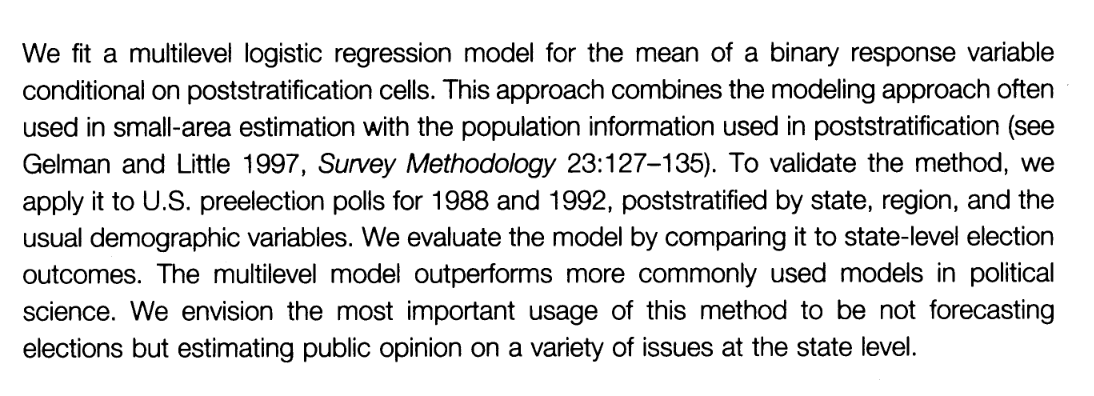
\includegraphics[width=\textwidth]{figures/park_bayesian_2004_abstract}}
\end{center}

\vfill
\url{https://www.jstor.org/stable/25791784} \\ See also Gelman and Hill (2007), Chapter 14 (``Multilevel logistic regression'')

\end{frame}
%%%%%%%%%%%%
\begin{frame}{Mr. P.}

$\hat{\bar{y}}_h$ comes from an individual-level model

\begin{align*}
Pr(y_i = 1) = logit^{-1} (\beta_0 + \\
 \beta_{male} \cdot male_i + \\
 \alpha_{k[i]}^{age} + \\
 \alpha_{k[i]}^{race} + \\
 \alpha_{k[i]}^{region})
\end{align*}

\begin{align*}
\alpha_{k}^{age} \sim N(0, \sigma^2_{age}) \text{ for } k = 1, \ldots, 4 \\
\alpha_{k}^{race} \sim N(0, \sigma^2_{race}) \text{ for } k = 1, \ldots, 5 \\
\alpha_{k}^{region}  \sim N(0, \sigma^2_{region}) \text{ for } k = 1, \ldots, 4
\end{align*}

Priors determined by RStanarm (\url{https://cran.r-project.org/web/packages/rstanarm/vignettes/priors.html})

\end{frame}

% Talk about two models fighting, shrinking coefficients toward 0
%%%%%%%%%%%%
%%%%%%%%%%%%%%
\begin{frame}{To learn more about Mr. P.}

{\footnotesize
Generally optimistic:
\begin{itemize}
\item Park, Gelman, and Bafumi. 2004. ``\textcolor{blue}{\href{https://www.jstor.org/stable/25791784}{Bayesian Multilevel Estimation with Poststratification: State-Level Estimates from National Polls}}.'' \textit{Political Analysis}.
\item Lax and Phillips. 2009. ``\textcolor{blue}{\href{https://www.jstor.org/stable/25193870}{How should we estimate public opinion in the states?}}'' \textit{American Journal of Political Science}.
\item Ghitza and Gelman. 2013. ``\textcolor{blue}{\href{https://www.jstor.org/stable/23496652}{Deep Interactions with MRP: Election Turnout and Voting Patterns Among Small Electoral Subgroups}}.'' \textit{American Journal of Political Science}.
\item Warshaw and Rodden. 2012. ``\textcolor{blue}{\href{http://www.jstor.org/stable/10.1017/s0022381611001204}{How should we measure district-level public opinion on individual issues?}}'' \textit{Journal of Politics}.
\item Downs et al. 2018. ``\textcolor{blue}{\href{https://doi.org/10.1093/aje/kwy070}{Multilevel Regression and Poststratification: A Modelling Approach to Estimating Population Quantities From Highly Selected Survey Samples}}.'' \textit{American Journal of Epidemiology}.
\end{itemize}
Generally cautious:
\begin{itemize}
\item Buttice and Highton. 2013. ``\textcolor{blue}{\href{http://www.jstor.org/stable/24572674}{How Does Multilevel Regression and Poststratification Perform with Conventional National Surveys?}}'' \textit{Political Analysis}.
\end{itemize}
}

\end{frame}
%%%%%%%%%%%%%%%%%%%%%%%%%%
\begin{frame}{Notes}

\begin{itemize}
\item Modeling allows you to make more estimates for smaller groups \pause
\item These techniques is widely used by modern pollsters (e.g., YouGov) and political scientists \pause
\item You will not finish this activity.  That's OK.

\end{itemize}
%%%%%%%%%%%%%%%%%%%
\end{frame}
\begin{frame}

Our recommended work flow:
\begin{itemize}
\item Create a write-up that describes what data you will be collecting, why, and how it will be shared with others (for tips, see \href{https://doi.org/10.1177/2515245917747656}{Meyer})
\item Create survey on Google Forms
\item Deploy to MTurk
\item Take a break
\item Validate and pay workers
\item Analyze the much larger sample that we have collected for you
\item De-identify and ``open-source'' data by sending to your local organizer (but remember to think about the end at the beginning)
\end{itemize}

\end{frame}
%%%%%%%%%%%%%%%%%%%%%%%%%%
\begin{frame}

\begin{figure}
  \centering
  
\includegraphics[width=0.9\textwidth]{figures/pandas_video}
\end{figure}

\url{https://www.youtube.com/watch?v=66oNv_DJuPc}

\end{frame}
%%%%%%%%%%%%%%%%%%%%%%%%%%%%%%%%
\begin{frame}

Brief introduction into open-sourcing your data:
\begin{itemize}
\item Store your data in a simple format
\pause
\item Provide documentation
\pause
\item Beware of privacy
\end{itemize}

\end{frame}
%%%%%%%%%%%%%%%%%%%%%%%%%%
\begin{frame}
\frametitle{Store your data in a simple format}

\pause
In this case .csv should be good.

\end{frame}
%%%%%%%%%%%%%%%%%%%%%%%%%%%
\begin{frame}
\frametitle{Provide documentation}

\pause
What would another researcher want to know? 

\begin{itemize}
\item How and when was this data collected?
\item What do the different variables describe?
\end{itemize}

\end{frame}
%%%%%%%%%%%%%%%%%%%%%%%%%%%
\begin{frame}
\frametitle{Provide documentation (more details)}

\begin{figure}
  \centering
  
\includegraphics[width=0.9\textwidth]{figures/icpsr_metadata}
\end{figure}

\vfill
\url{https://www.icpsr.umich.edu/icpsrweb/content/deposit/guide/chapter3docs.html}

\end{frame}
%%%%%%%%%%%%%%%%%%%%%%%%
\begin{frame}
\frametitle{Beware of privacy}

Risks come from combining data sources\\

\vfill

\begin{minipage}[c]{0.35\textwidth}
$\underbrace{\text{Baking soda}}_{\text{Safe}} + \underbrace{\text{Vinegar}}_{\text{Safe}} =$
\end{minipage}
\hspace{0.05\textwidth}
\begin{minipage}[c]{0.55\textwidth}
\onslide<2>{
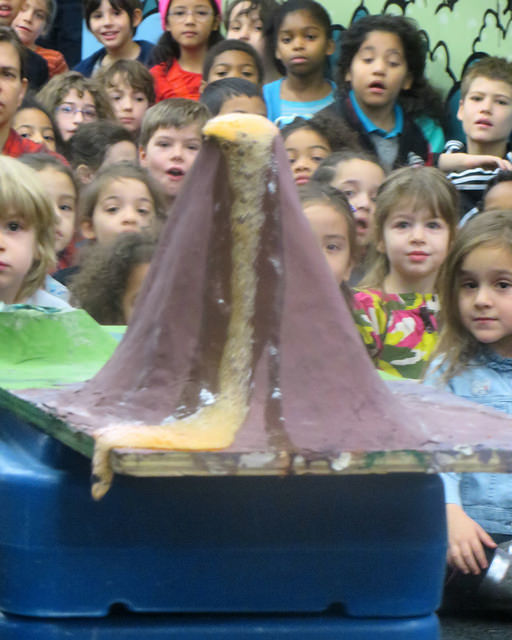
\includegraphics[width=0.6\textwidth]{figures/baking_soda_volcano}\\ {\tiny \url{https://www.flickr.com/photos/edenpictures/15962352215/}}
}
\end{minipage}

\end{frame}
%%%%%%%%%%%%%%%%%%%%%%%%%%

\begin{frame}
\frametitle{Beware of privacy}

Remove personally identifying information and information that can be used for linking

\begin{figure}
  \centering
  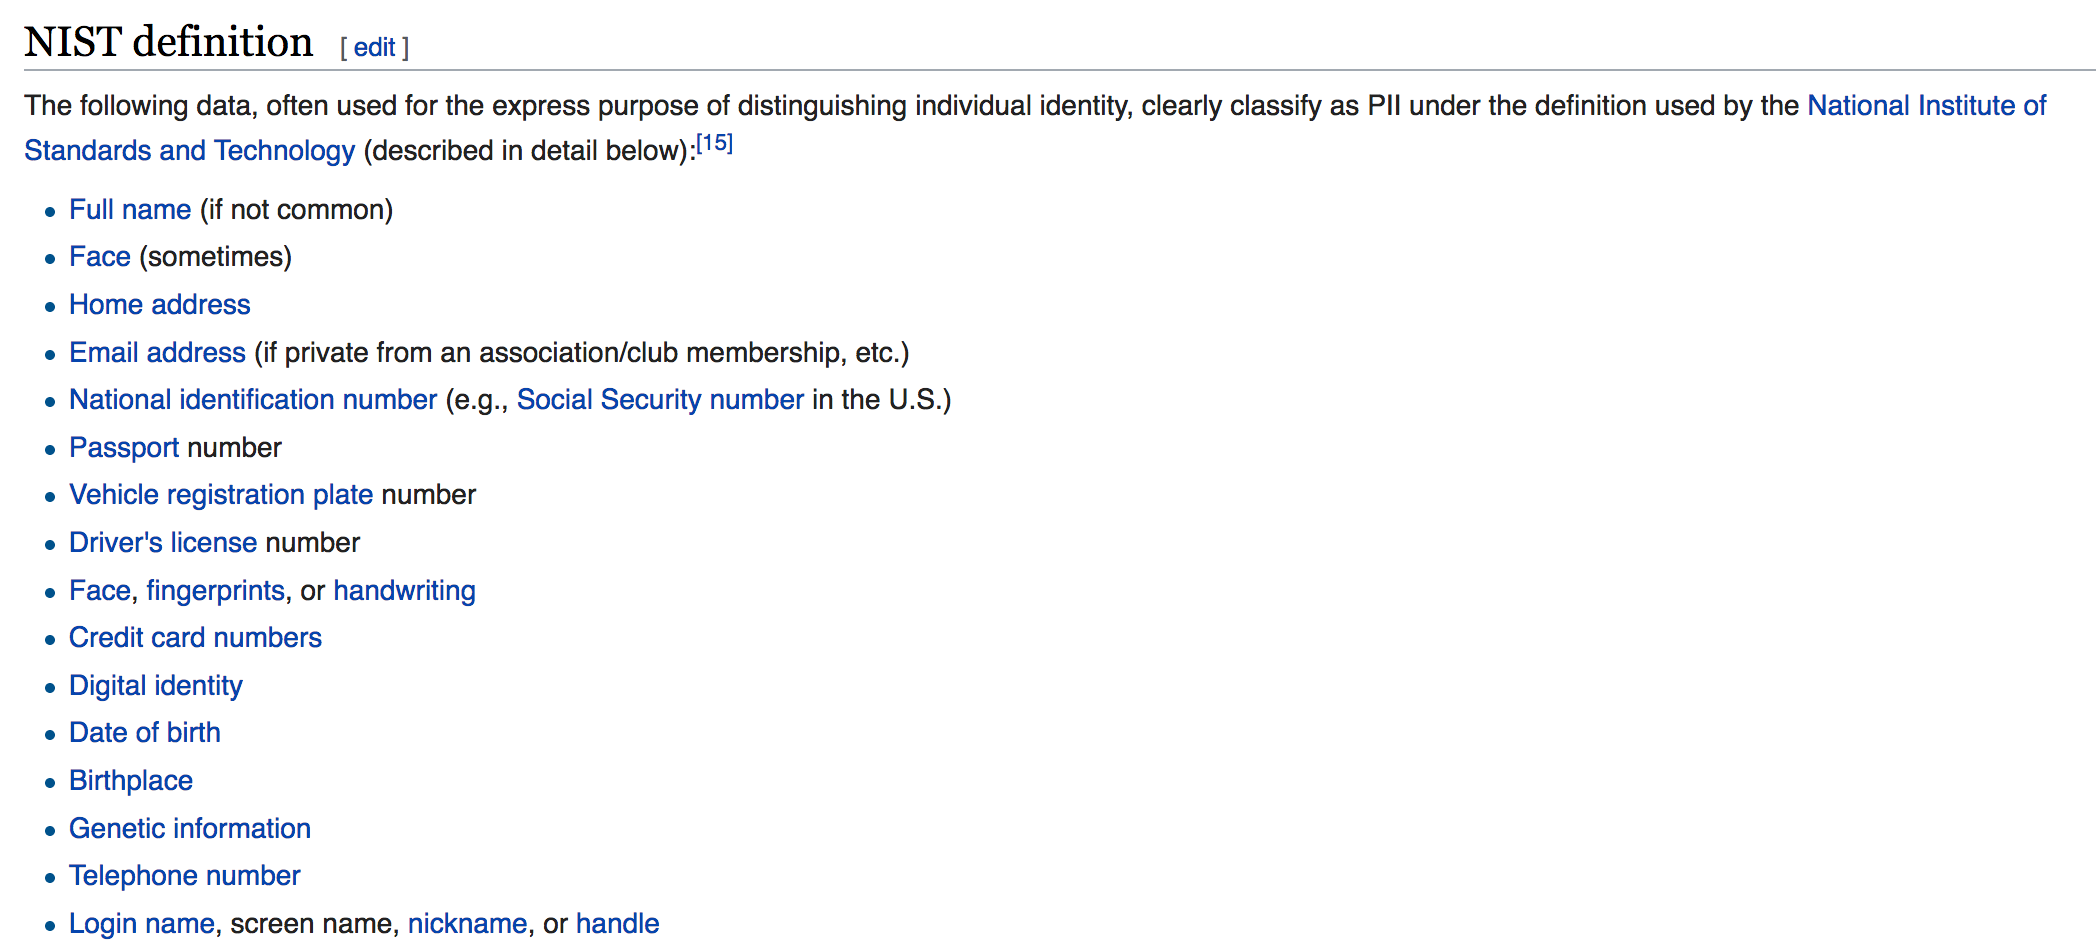
\includegraphics[width=0.9\textwidth]{figures/pii_nist}
\end{figure}

\vfill
\url{https://en.wikipedia.org/wiki/Personally_identifiable_information}

\end{frame}
%%%%%%%%%%%%%%%%%%%%%%%%
\begin{frame}

\begin{figure}
  \centering
  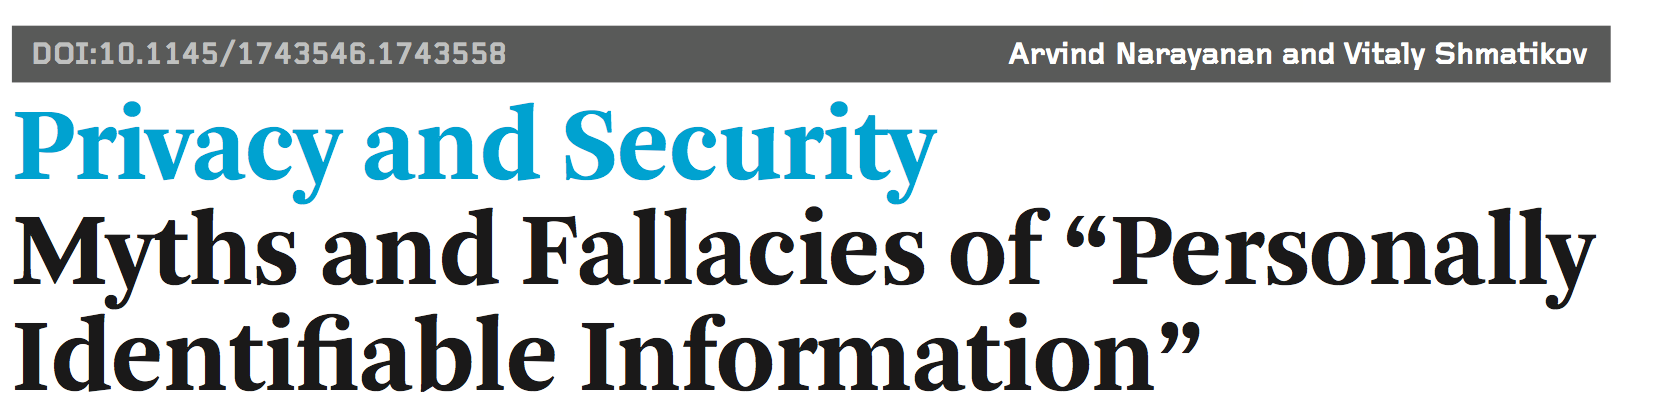
\includegraphics[width=0.9\textwidth]{figures/narayanan_myths_2010_title}
\end{figure}

\vfill
\url{http://dx.doi.org/10.1145/1743546.1743558}
\end{frame}
%%%%%%%%%%%%%%%%%%%%%
\begin{frame}

In this case, we recommend:
\begin{itemize}
\item Removing PII (name, email address, etc)
\item Removing TurkID
\item Coarsen age, geography, and race/ethnicity
\item Coarsen timestamp
\item Anything else?
\end{itemize}

For more on coarsening, see this code:\\
\url{https://github.com/compsocialscience/summer-institute/blob/master/2019/materials/day4-surveys/activity/mturk_data_cleaning.Rmd}

\end{frame}
%%%%%%%%%%%%%%%%%%%%%%%%%%
\begin{frame}

For more about de-identification, see 
\begin{itemize}
\item \textit{Bit by Bit}, Sec 6.6.2 \href{https://www.bitbybitbook.com/en/1st-ed/ethics/dilemmas/info-risk/}{\textcolor{blue}{``Understanding and managing informational risk''}}
\item Lundberg, Levy, Narayanan, Salganik (2019) ``\href{https://arxiv.org/abs/1809.00103}{Privacy, ethics, and data access: A case study of the Fragile Families Challenge'}'
\end{itemize}

\end{frame}
%%%%%%%%%%%%%%%%%%%%%%%%%%
\begin{frame}

The 5Ws of data release: \pause
\begin{itemize}
\item Who: You
\pause
\item What: make your data available to other researchers in a responsible way
\pause
\item Where: Dataverse, ICPSR, or an archival data repository \pause (your laptop is not an archival data repository)
\pause 
\item When:  when you publish your paper
\pause
\item Why: It is good for you and it is good for the world
\end{itemize}

\end{frame}
%%%%%%%%%%%%%%%%%%%%%%%%%%
\begin{frame}

Share your data to your local organizer who can post it here:\\
\url{https://github.com/compsocialscience/summer-institute/tree/master/2019/materials/day4-surveys/datasets}

\end{frame}
%%%%%%%%%%%%%%%%%%%%%%%%%%
\begin{frame}

When you start your projects next week
\begin{itemize}
\item plan to release your data
\item plan to release your code
\end{itemize}

\end{frame}
%%%%%%%%%%%%%%%%%%%%%%%%%%
\begin{frame}

\begin{center}
\LARGE Questions
\end{center}

\end{frame}
%%%%%%%%%%%%%%%%%%%%%%%%%%%
\begin{frame}

Our recommended work flow:
\begin{itemize}
\item Create a write-up that describes what data you will be collecting, why, and how it will be shared with others (for tips, see \href{https://doi.org/10.1177/2515245917747656}{Meyer})
\item Create survey on Google Forms
\item Deploy to MTurk
\item Take a break
\item Validate and pay workers
\item Analyze the much larger sample that we have collected for you
\item De-identify and ``open-source'' data by sending to your local organizer (but remember to think about the end at the beginning)
\end{itemize}

\end{frame}
%%%%%%%%%%%%%%%%%%%%%%%%%%

\end{document}
